\chapter{A New Kind of Disorientation}

My initial encounter with the forest sangha at Wat Pah Pong had left me
disappointed and confused. This second attempt had left me utterly
shattered. I think it is safe to say that my faith was undiminished but
certainly it was obscured. The pain of humiliation, failure and
loneliness were overpowering: so much sadness. At times it did actually
feel as if my sense of identity had literally been shattered -- as if my
conventional sense of self had broken. I wondered what I was going to
have to do to reconstruct a functioning sense of self. It was evident
that the previous one had not been fit for purpose. This was not the way
I figured my spiritual journey might unfold.

At other times I had the powerful impression that my heart had been
scarred for eternity: that the depth and intensity of pain I'd suffered
had caused an irreversible wounding. The thought of my having made such
a massive mistake fed into my sense of failure and self-condemnation.
Even just thinking the thought `I', could trigger a fiery upthrust of
guilt, and these regular upthrusts were compounding self-doubt. There
was a strong suspicion that I felt this bad because I \emph{was} this
bad.

There wasn't anyone around who was particularly interested in what was
happening for me, so I was left alone to endure. Besides endurance,
though, there was still that underlying and significant sense of
belonging to a community. Maybe it was true that nobody was interested
in my miserable condition, but I was still part of something. I believe
this perception held me in a way that contributed to my not being
completely overwhelmed. Perhaps also, as a consequence of that shift in
perception of `abiding as the context of all experience', some sort of
rewiring of my mind had occurred and I was being afforded protection.
Faith is a mysterious matter; if we try too hard to understand it we
deny its reality.

Gratefully, one day Phra Somdet instructed a worker at the monastery to
give me the use during the day of one of the big, usually empty,
temples. It was vast, dark and ornate, similar to the large main temple
in which I had received my novice and monk's precepts. Certainly I
appreciated this gesture of thoughtfulness, but as it happened it did
little to placate the madness of my mind. There were times when I felt a
visceral hatred for anything to do with Buddhism; I think there were
occasions when I actually felt nauseous. Was this a purging of guilt, or
a release of previously denied resentments? I really didn't know.
Fortunately, that state of `not-knowing' was not the whole of me.
Although I continued to regularly be dragged down by a vortex of pain
into fiery hell realms, part of my mind was still able to contemplate.

In the evenings I was invited to sit with Phra Somdet in his private
meditation room upstairs in his kuti. I would go there after evening
puja and already be sitting by the time he arrived. A vivid mental image
has stayed with me of how he began with humbly bowing to the shrine,
then would sit back and lean against the wall. I imagine he was tired at
the end of a long day. Then, after perhaps five or so minutes, he would
shuffle forward, light the candles and incense and settle into
meditation. When I couldn't bear the pain in my knees any longer, I
would quietly leave the room, with Phra Somdet still sitting there.

There was a substantial library in Ganna Soung where I was staying, and
it was well stocked with books from various different Buddhist
traditions. I found myself wondering if I might be better off at
Song Kwang Sa\cite{song} monastery in Korea under Master Ku San, or perhaps going
to Japan. I still felt drawn to Japan. Given the state of my knees
though, and the long periods of obligatory group sitting meditation
practised in those traditions, I recognized those options were not
realistic. Also, I think I was wondering about the training in
\emph{vinaya}. In the midst of all the turmoil I was having to endure, I
like to think I was still able to appreciate the importance of a strict
training in discipline and restraint. Probably there was uncertainty as
to whether such a training was going to be available elsewhere. So my
fantasies were never more than that: stories I was telling myself as I
puzzled over what I was supposed to be doing with my life.

As one week flowed into another, it felt like I was in survival mode: so
much fear, so much loneliness and no sense of direction. One day, I
think around the end of 1975, there was a knock on the door of my room
at Ganna Soung: it was Tan Jotiko, previously known as Nane Dhammiko,
previously known as Bill Hamilton. Once more, he was accompanying Ajahn
Sumedho and they were staying at Wat Saket. Certainly I was keen to meet
Ajahn Sumedho again. When we did meet, Ajahn Sumedho spoke
enthusiastically about the new monastery they were involved in building.
Not long after I had left Wat Pah Pong the year before, he and a group
of Western monks had been invited to set up a monastery in a forested
area just outside the village of Bahn Bung Wai. The group had spent the
Rains Retreat of 1975 there, and it now looked like a monastery called
Wat Pah Nanachat (the International Forest Monastery) was well on the
way to being established. I imagine the idea appealed to me; however, I
was still cautious. The main thing I took away from that conversation
with Ajahn Sumedho was his response to something I said just as I was
about to leave and go back to Wat Boworn. I had told him how I had been
feeling terribly torn because I really wanted to live the life of a
forest monk, but after the experience at Wat Hin Maak Peng, felt
uncertain as to whether or not I would be able to do it. `Maybe I should
try and learn to practise in a city monastery', I had said to him.
`Besides, the idea that practising in the forest monasteries is better
than practising in a city monastery, is just an opinion, and Tan Ajahn
Chah strongly emphasizes we shouldn't attach to views and opinions'.
Ajahn Sumedho responded with a big smile and said, `Yes, that is true,
however some opinions are right'.

Around the beginning of 1976 my dear friend from New Zealand, Jutta
Passler, came to visit. She was on her way to spend time in India but
had planned a stop-over in Bangkok. How fortunate. Her friendship was
very healing. We didn't really discuss the disintegration taking place
within me, but having her company was like a balm. I am reminded of what
the Buddha said about \emph{kalyanamitta}. Jutta was indeed a wonderful
\emph{kalyanamitta}.

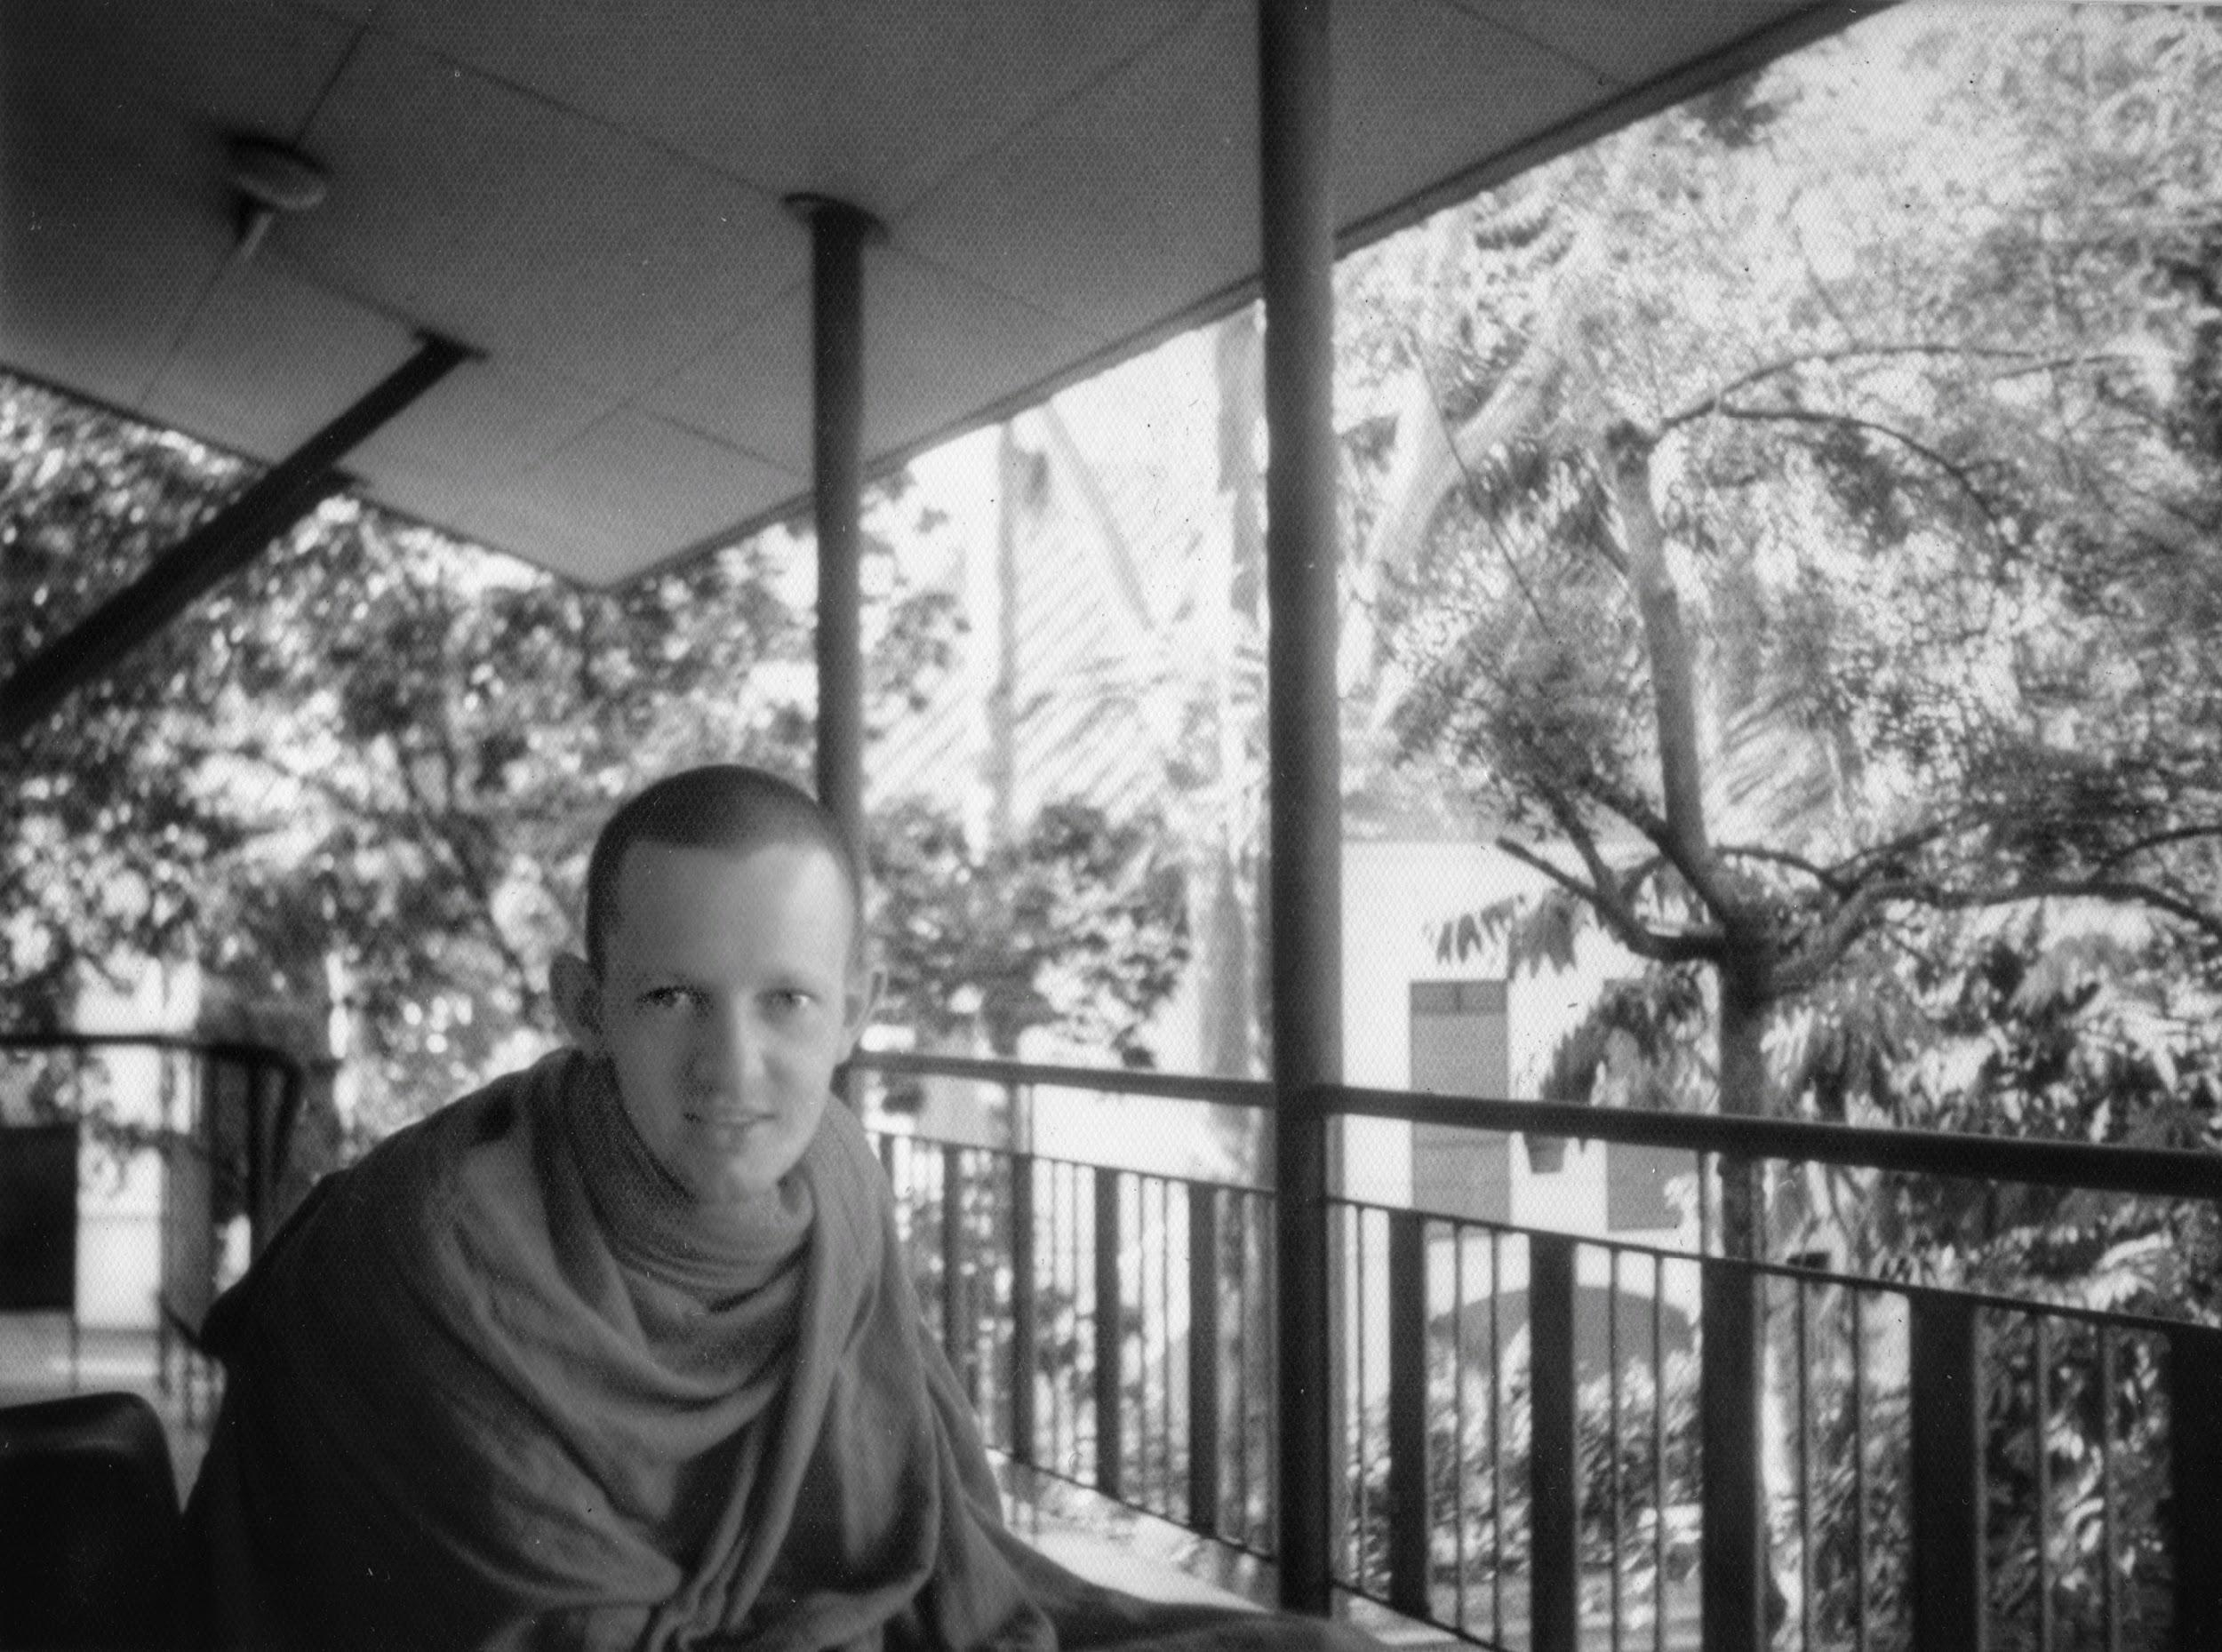
\includegraphics[width=\linewidth]{image1.jpeg}

During the time Jutta was visiting, Tan Jotiko again turned up at my
door, this time he was in Bangkok to see his parents off back to
America; they had been visiting him at Wat Pah Nanachat. He was
enthusiastic about me at least coming to visit the new monastery.
Probably I was already thinking about the potential conflict between Tan
Ajahn Chah's monastery being part of the Mahanikaya Sect and myself
having taken Precepts in the Dhammayutta Sect, but by now the invitation
to visit had become appealing, so a plan was hatched for the three of
us, including Jutta, to take the train to Ubon.

